\section{Cryptographic Hash Functions}\label{sec:cryptopgrahic-hash-functions}

In the previous section, Merkle trees were discussed in detail, with particular attention to the use of cryptographic hash functions for node construction.  
One of the questions that emerged during my internship was: \emph{``what is the fastest cryptographic hash function?''}.  
% Although it is difficult to provide a definitive answer to this question, the Rust implementation of Merkle trees that I developed and published on \texttt{crates.io} was designed to be flexible.  
% Specifically, it relies on a trait-based abstraction that allows the integration of different hash functions depending on the desired use case.

% The current version of \texttt{mt-rs}\footnote{\url{https://crates.io/crates/mt-rs}} includes support for three hash functions: SHA-256, Keccak-256, and BLAKE3.  

This section explores the motivation behind testing different cryptographic hash functions (SHA-256, Keccak-256, and BLAKE3) within the context of this project and why, among these, BLAKE3 was selected as the primary candidate for benchmarking in this thesis due to its performance and modern design.  

\subsection{SHA-256}

SHA-256 is part of the SHA-2 family of cryptographic hash functions, standardized by NIST in 2001 \cite{penard2008secure}.
It produces a 256-bit output from input messages of arbitrary length and is widely used in security protocols such as TLS, digital signatures, and blockchain systems like Bitcoin.

The algorithm processes data in 512-bit blocks using 32-bit words. On 32-bit architectures, this design choice makes SHA-256 relatively efficient. However, on modern 64-bit CPUs, the reliance on 32-bit operations leads to extra instructions, making it slower than SHA-512 and significantly less efficient than more modern designs such as BLAKE3. By contrast, SHA-512 processes 1024-bit message blocks with 64-bit operations, making it more efficient on such architectures. In this thesis, however, SHA-512 was not benchmarked, as the focus was on SHA-256 and the comparison against Keccak-256 and BLAKE3.

Despite these performance limitations, SHA-256 remains a cornerstone in cryptography due to its simplicity, standardization, and lack of practical vulnerabilities. It is often used as a reference point in performance evaluations of newer hash functions.

\subsection{Keccak-256}

Keccak-256 \cite{bertoni2013keccak} is the 256-bit variant of the Keccak family, which won the NIST SHA-3 competition in 2012 \cite{nist-sha3}. Unlike SHA-2, Keccak is based on a \emph{sponge construction} that alternates between absorbing input blocks and squeezing output. This design provides strong theoretical guarantees and a high level of security against known cryptanalytic attacks.  

Although Keccak-256 is cryptographically very robust, its performance is generally slower than SHA-2 and significantly slower than BLAKE3 in software implementations. However, its adoption is widespread in domains where security guarantees are paramount. A prominent example is Ethereum, where Keccak-256 is used extensively in transaction validation, block hashing, and smart contract execution.  

In this thesis, Keccak-256 is included not because of raw speed but because of its relevance in production distributed systems, where it demonstrates the trade-off between cryptographic strength and computational efficiency.

\subsection{BLAKE3}

The BLAKE3 cryptographic hash function \cite{blake3-oconnor} is an evolution of the BLAKE2 cryptographic hash function \cite{aumasson2013blake2}, providing higher performance and introducing several additional features:
\begin{itemize}
    \item Support for hashing, keyed hashing, and key derivation modes.
    \item No additional space cost for keyed hashing.
    \item Parallelizable output generation.
\end{itemize}

BLAKE3 employs a binary tree structure that splits the input into 1024-byte chunks, which are treated as the leaves of the tree. The final chunk may be shorter, but it cannot be empty (unless the entire input is empty). This design enables unlimited parallelism, as each chunk can be compressed independently, allowing efficient use of modern CPUs with SIMD instructions.

BLAKE3 achieves significantly better performance than both SHA-256 and SHA-512 on modern 64-bit architectures. Within the SHA family, SHA-512 generally outperforms SHA-256 on 64-bit machines \cite{gueron2011sha}. 

BLAKE3's superior performance derives from its fundamentally different design philosophy. Unlike the inherently sequential SHA algorithms, its tree-based parallelism, fewer rounds, more efficient mixing function, and better cache locality enable it to outperform both SHA variants regardless of word size alignment considerations.

It provides a 128-bit security level and a 256-bit output.

Formally, for a message of length $n > 1024$ bytes, the left subtree covers a number of bytes equal to:

\[
2^{10 + \lfloor \log_2{\left(\frac{n-1}{1024}\right)} \rfloor}
\]

The right subtree consists of the remainder. BLAKE3 supports input of any length $0 \leq \ell < 2^{64}$.

This section does not aim to describe the full BLAKE3 specification (e.g., its compression function or internal modes of operation), but rather to emphasize its practical performance benefits in the context of this work.

\subsubsection{Performance}

Figures \ref{fig:blake3-thoughput-example} and \ref{fig:blak3-speed} show benchmark results from an AWS \texttt{c5.metal} instance equipped with dual Intel Xeon Platinum 8275CL (Cascade Lake-SP) processors supporting AVX-512.  
These results highlight BLAKE3's superior performance compared to other widely used hash functions.

\begin{figure}
    \centering
    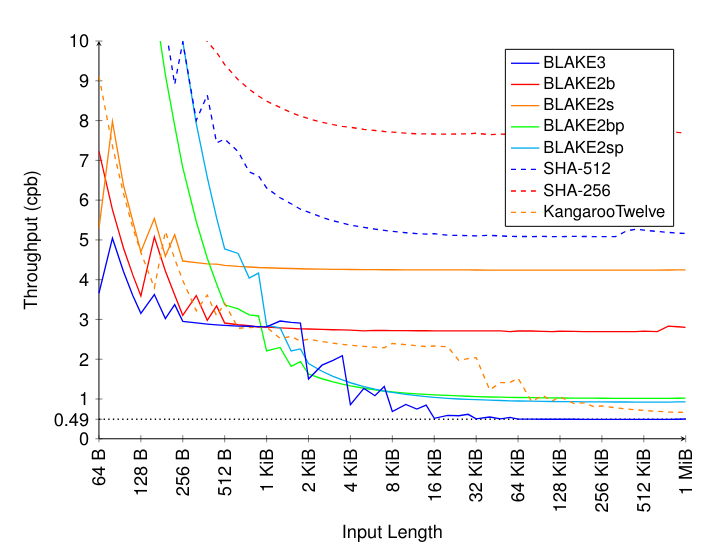
\includegraphics[width=0.7\linewidth]{assets/blake3-throughput-example.png}
    \caption{Single-threaded throughput of BLAKE3 and other hash functions on an AWS c5.metal
instance, measured in cycles per byte (cpb). Lower values indicate fewer CPU cycles needed per byte.}
    \label{fig:blake3-thoughput-example}
\end{figure}

\begin{figure}
    \centering
    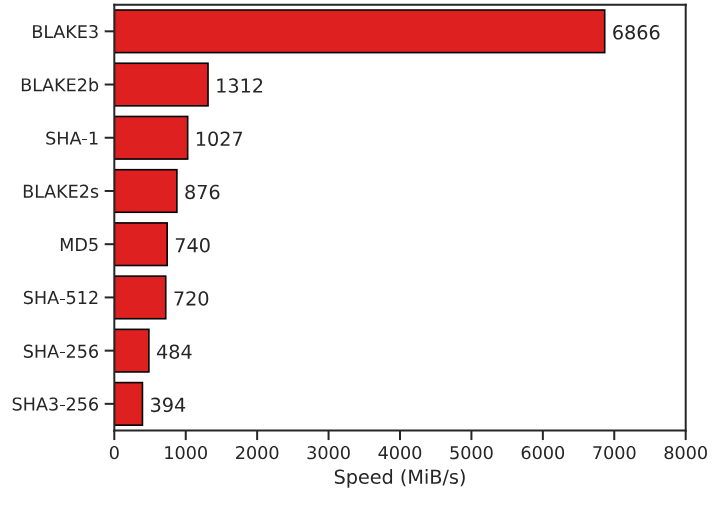
\includegraphics[width=0.7\linewidth]{assets/blake3-speed.png}
    \caption{Hashing speed comparison of BLAKE3 and other hash functions on an AWS c5.metal instance
with a 16~KiB input, using a single thread. Higher values (MiB/s) indicate faster processing.}
    \label{fig:blak3-speed}
\end{figure}

In the context of this thesis, benchmarks were also conducted using the
\texttt{mt-rs}\footnote{\url{https://crates.io/crates/mt-rs}} library to evaluate Merkle tree creation and proof generation under these three different cryptographic hash functions.  
For each function, three tests were performed with node data sizes of 5 MB, 10 MB and 15 MB.  
In each test, the benchmark measures the time required to construct the authentication path for a leaf, verify the corresponding root from that path, and repeat this process for all 10 nodes of the Merkle tree.

The results, reported in Table \ref{tab:benchmarks-hash-functions}, demonstrate that BLAKE3 consistently outperforms both SHA-256 and Keccak-256 in terms of execution time.

\begin{table}[h!]
    \centering
    \begin{tabular}{|l|c|c|c|}
    \hline
       \textbf{Hash function} & \textbf{5 MB} & \textbf{10 MB} & \textbf{15 MB} \\
       \hline
        SHA-256 & 89.901 ms & 178.42 ms & 268.53 ms \\
        Keccak-256 & 521.49 ms & 1.1334 s & 1.3438 s \\
        BLAKE3 & 73.091 ms & 154.68 ms & 219.79 ms \\
        \hline
    \end{tabular}
    \caption{Merkle tree benchmarks with 10 nodes per dataset size (5 MB, 10 MB, and 15 MB).}
    \label{tab:benchmarks-hash-functions}
\end{table}
